\documentclass[12pt]{article}
\usepackage{algorithm2e}
\usepackage{latexsym}
\usepackage{amssymb,amsmath}
\usepackage[pdftex]{graphicx}
\usepackage{listings}
\usepackage{xcolor}
\usepackage{amsmath}
\lstset{language=R,basicstyle=\scriptsize\ttfamily,commentstyle=\ttfamily\color{gray},frame=single,breaklines=true,keepspaces = true,keywordstyle=\color{red},xleftmargin=-10mm}

\topmargin = 0.1in \textwidth=5.7in \textheight=8.6in

\oddsidemargin = 0.2in \evensidemargin = 0.2in

\usepackage{graphicx}
\graphicspath{ {"/Users/hogstrom/Dropbox (Personal)/cources_spring_2015_MIT/18_335_Numeric_Methods/NMF/figures/"} }
\DeclareGraphicsExtensions{.pdf,.png,.jpg}

\usepackage{amsmath}

\begin{document}

Larson Hogstrom 

MIT 18.335

Final Project

April 16, 2015 \\


\begin{equation}
    \min_{W \ge 0} || \left( \begin{array}{c} H^T   \\  \sqrt{\alpha_W}I_k \\ \end{array} \right) W^T- \left( \begin{array}{c} A^T   \\  0_{kxm} \\ \end{array} \right) ||^{2}_{F} 
\end{equation}

\begin{equation}
    \min_{H \ge 0} || \left( \begin{array}{c} W   \\  \sqrt{\alpha_H}I_k \\ \end{array} \right) H- \left( \begin{array}{c} A   \\  0_{kxm} \\ \end{array} \right) ||^{2}_{F} 
\end{equation}


\textbf{Outline}

-Introduction + definition

-cost functions: Euclidian distance, Frobinius norm, KL divergence, Renyi's divergence. Can you construct a situation in which certain norms are better than others?

-update rules: multiplicative update, ALS method, gradient methods

-computational comparison: flop counts, accuracy, size of inputs

-applications to calculating metagenes \\

To date, 
Iterative algorithms, for example, build factorized components while converging on a local minimum of a specified object function. 

-problem with NMF - no unique solution 
In NMF, a low ran approximation of an input data matrix A is created with smaller, non-negative factors called W and H. 
In the case of gene expression and other biological phenomena 

This project compares multiple algorithms for computing NMF factorization including gradient and non gradient methods. The motivation 
fixed-point type methods 
minimization problem with bounded constraints 

\textbf{Introduction} \\
This report introduces the framework for parts-based representations using NMF and focuses on the algorithms and numerical aspects of computation. \\

\textbf{definition} For a nonnegative matrix $\bf{A} \in \mathbb{R}^{m x n}$, select a low-rank approximation of size k such that there are two nonnegative matrices \textbf{W} $ \in \mathbb{R}^{m x k}$ and \textbf{H} $ \in \mathbb{R}^{k x n}$ which minimizes a function such as 
$$ f( \textbf{W,H}) = \frac{1}{2} || \textbf{A - WH} || ^{2}_{F}$$


Other commonly used objective functions include Euclidian distance and Kullback-Leibler (KL) divergence. KL can be extended to a more general information-based framework using Renyi's divergence. (Devarajan, 2005). Here, a single parameter $\alpha$ is used to represent a continuum of distance measures and KL airises as a special case as $\alpha \to 1$. 

$$ KL(V || WH) = \sum_{ij}{[V_{ij} \log{ \frac{V_{ij}}{(WH)_{ij}} - V_{ij} + (WH)_{ij}} ]} $$

more text

\pagebreak 

\textbf{Fundamental Algorithms} \\

One of the first and most widely adopted algorithms for NMF is the multiplicative update rule. This takes the general form: \\


\begin{algorithm}[H]
 \KwData{Input data matrix:  $\bf{A} \in \mathbb{R}^{m x n}$}
 \KwResult{nonnegative factorization of \textbf{A} using k components, creating matrices \textbf{W} $ \in \mathbb{R}^{m x k}$ and \textbf{H} $ \in \mathbb{R}^{k x n}$ }

 initialization\;
$\bf{W} \gets $ random dense (m x k) matrix\\
$\bf{H} \gets $ random dense (k x n) matrix\\
 \For{i = 1 to \text{maxiter} }{
 	$\bf{H = H .* (W^T A) ./ (W^T WH)} $
	
 	$\bf{W = W .* (A H^T) ./ (WHH^T)} $	}
 \caption{multiplicative update}
\end{algorithm} 


Often the \\
requires O(mnk) work per iteration

\begin{figure}[h!]
  \caption{A picture of a gull.}
  \centering
    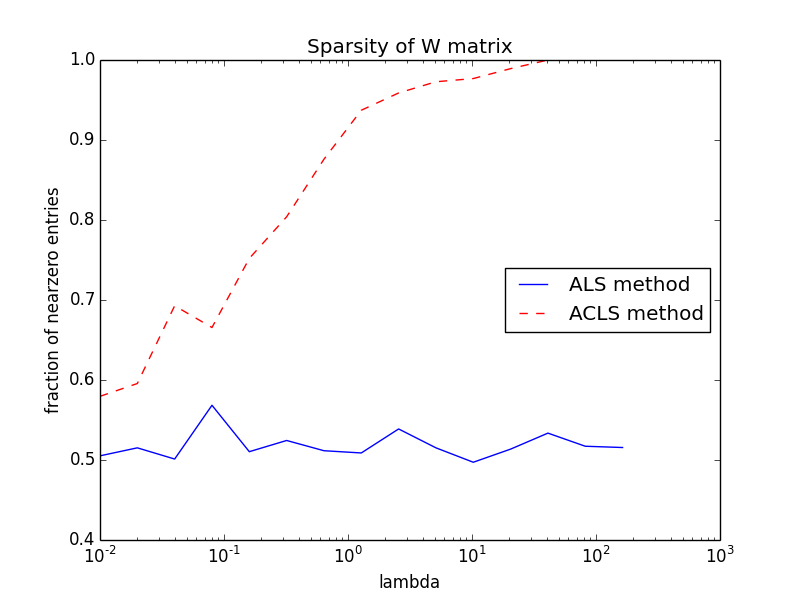
\includegraphics{ALS_vs_ACLS_sparsity}
\end{figure}



\end{document}